%! Author = mddzi
%! Date = 02.06.2024

% Preamble
% czcionka zgodna z wytycznymi to 10pt
\documentclass[12pt,a4paper,twoside]{report}

% Packages
\usepackage{amsmath}
\usepackage[T1]{fontenc}
\usepackage[utf8]{inputenc}
\usepackage{lmodern}
\usepackage{textcomp}
%\usepackage{lastpage}
\usepackage[inner=3.5cm,outer=2.5cm,top=2.5cm,bottom=2.5cm]{geometry} % margines zgodny z wytycznymi
%\usepackage[margin=3.5cm]{geometry} % margines oryginalny
\usepackage{graphicx}
\usepackage{fancyhdr}
\usepackage[svgnames]{xcolor}
\usepackage[font={small,color=Grey},labelsep=period,width={0.8\textwidth}]{caption}
\usepackage{float}
\usepackage{multirow}
\usepackage{subcaption}
\usepackage{adjustbox}
\usepackage{longtable}
\usepackage{etoolbox}
\usepackage{hyperref}
\usepackage{pdfpages}
\usepackage{indentfirst}
\usepackage{icomma}
\usepackage{natbib}
\usepackage{microtype}
\usepackage{url}
\usepackage{calc}
\usepackage{enumitem}
\usepackage{listings}
%\usepackage{lstmisc}
%\usepackage[backend=bibtex, sorting=none]{biblatex}

% set url breaks
\def\UrlBreaks{\do\/\do-}

% figures count
%\counterwithout{figure}{chapter}

% specified names
\renewcommand{\figurename}{Rysunek}
\renewcommand{\chaptername}{Rozdział}
\renewcommand{\tablename}{Tabela}
\renewcommand{\abstractname}{Streszczenie}
\renewcommand{\contentsname}{Spis treści}
\renewcommand{\bibname}{Bibliografia}
\renewcommand{\listfigurename}{Spis rysunków}
\renewcommand{\listtablename}{Spis tabel}

\renewcommand{\baselinestretch}{1.1} % interlinia oryginalna
%\renewcommand{\baselinestretch}{1.5} % interlinia zgodna z wytycznymi
\setlength{\parindent}{1.25cm} % wcięcie akapitowe zgodne z wytycznymi

%\renewcommand{\rmdefault}{phv} % Arial
%\renewcommand{\sfdefault}{phv} % Arial

% custom compact enumarate
\newenvironment{cenumerate}
{ \begin{enumerate}[itemsep=5pt,topsep=5pt,parsep=0pt] }
{
    \end{enumerate}
    \vspace{5pt}
}

% custom compact itemize
\newenvironment{citemize}
{ \begin{itemize}[itemsep=5pt,topsep=5pt,parsep=0pt] }
{
    \end{itemize}
    \vspace{5pt}
}

% custom comands
\newcommand{\todo} % command for TODO
{
    \textcolor{magenta}{\textit{\textbf{TODO}}}
}
\newcommand{\um}{\text{$\mu$m}} % command for micrometer

\newcommand{\incomment}[1] % command for inline comment
{
    \textcolor{magenta}{\textit{#1}}
}

% Listings style
\lstset{
    basicstyle=\ttfamily\footnotesize,
    breaklines=true,
%    frame=single,
    numbers=left,
    numbersep=5pt,
    numberstyle=\tiny\color{gray},
    showstringspaces=false,
    tabsize=1
}

% Url style
\urlstyle{same}

% Header and footer
\fancyhf{}
\fancyhead{}
\fancyhead[L]{Maksymilian Dziemiańczuk}
\fancyhead[R]{Projekt inżynierski}
%\fancyhead[RO,LE]{\footnotesize Program do tworzenia schematów układów scalonych w formie gry edukacyjnej}
\fancyfoot{}
\fancyfoot[RO,LE]{\thepage}
\fancyfoot[RE,LO]{\footnotesize Program do tworzenia schematów układów scalonych w formie gry edukacyjnej}
\fancypagestyle{plain}{
    \renewcommand{\headrulewidth}{0pt}
    \fancyhf{}
    \fancyfoot[RO,LE]{\thepage}
    \fancyfoot[RE,LO]{\footnotesize Program do tworzenia schematów układów scalonych w formie gry edukacyjnej}
}

% set pagestyle
\pagestyle{fancy}

% Document
\begin{document}

% title page
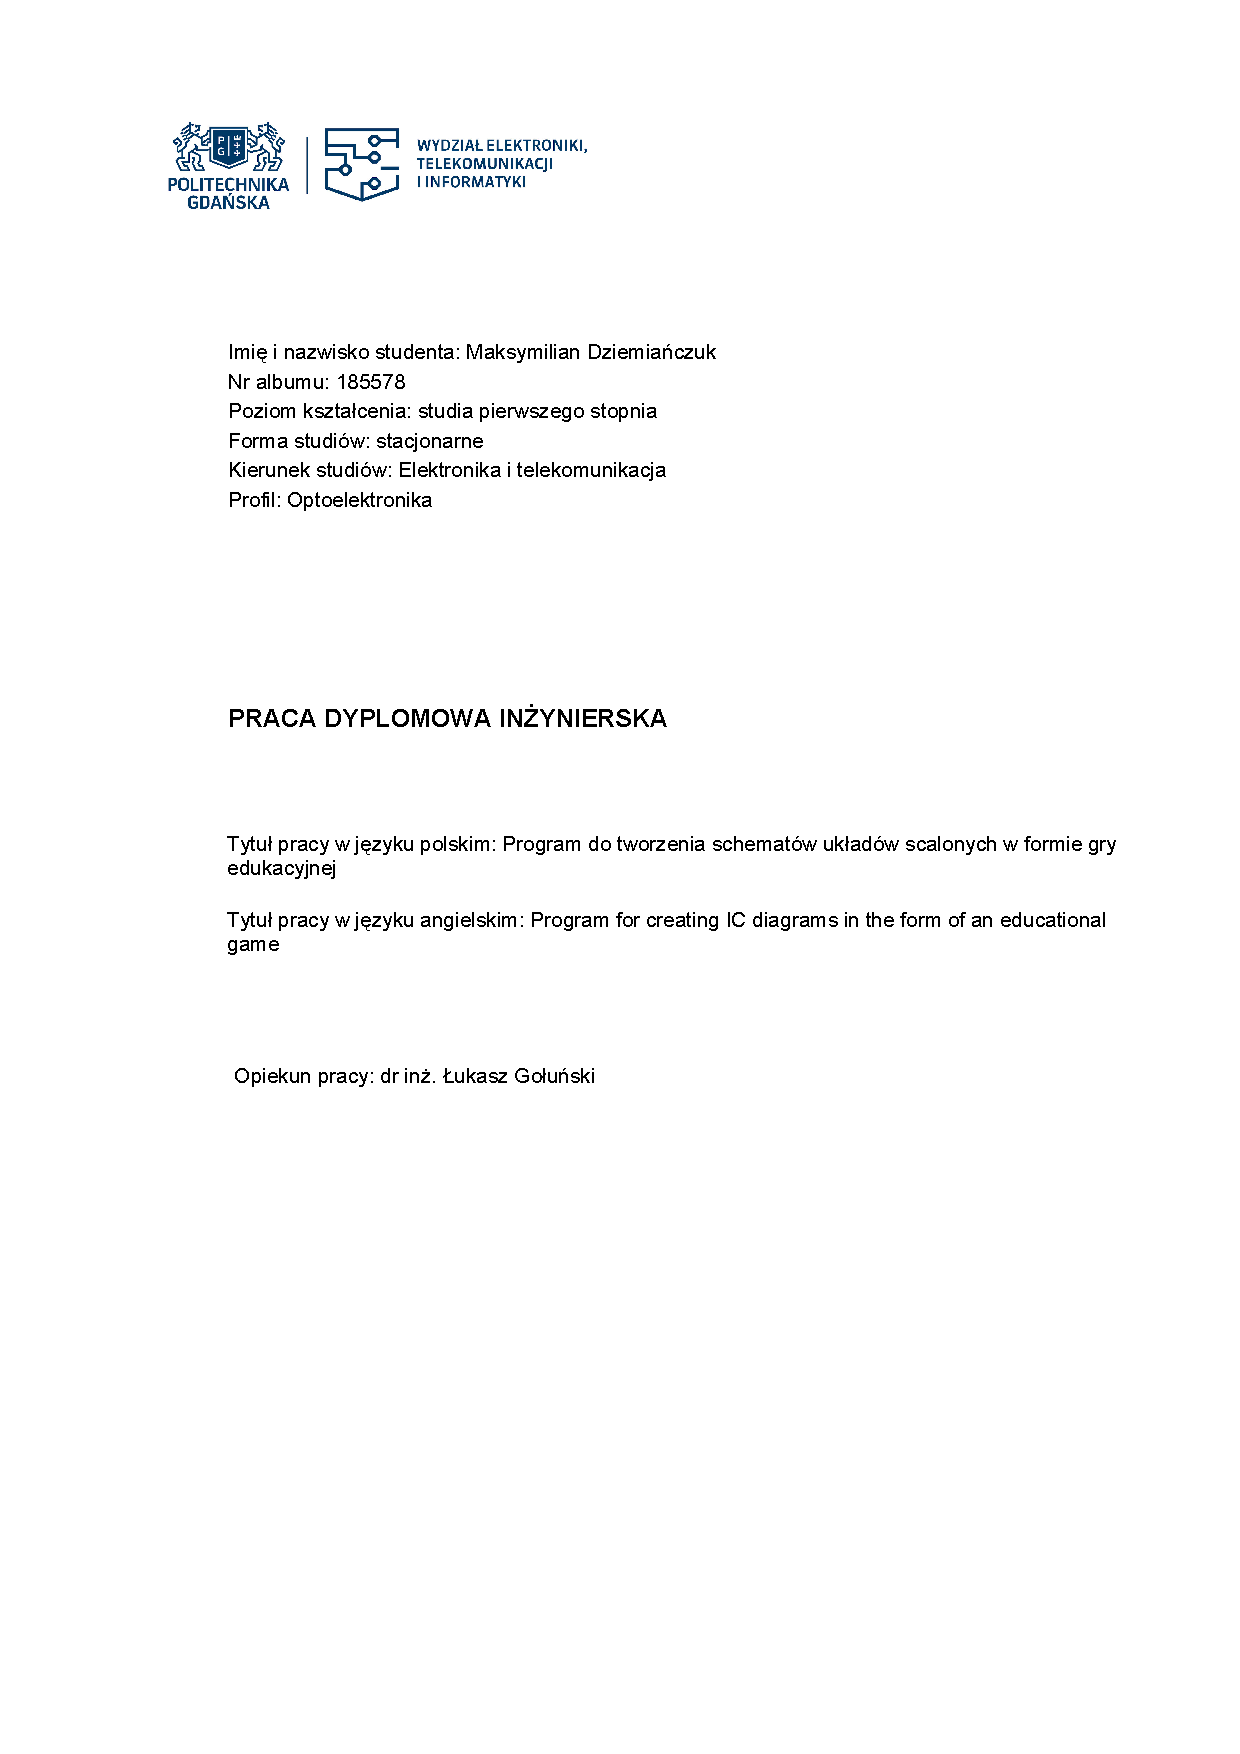
\includepdf[pages={1}]{StronaTytulowa_185578.pdf}

% empty page
\newpage \thispagestyle{empty} \ \newpage

\section*{Streszczenie}
\label{sec:streszczenie}
\thispagestyle{plain}
%\abstract
Celem niniejszej pracy jest opracowanie edukacyjnej gry komputerowej umożliwiającej wprowadzenie użytkownika
w~zagadnienia projektowania schematów układów scalonych,
z~wykorzystaniem silnika Unity i~języka C\#.
Aplikacja stanowi narzędzie zarówno do nauki,
jak~i~praktycznego ćwiczenia podstawowych koncepcji projektowania w~interaktywnej formie,
łącząc aspekty edukacyjne z~rozrywką.\\
\indent %Do realizacji projektu przyjęto architekturę MVVM (Model-View-ViewModel),
%która zapewnia modularność oraz przejrzystość kodu,
%umożliwiając łatwe utrzymanie i~przyszłe rozszerzenia aplikacji.
Kluczowym elementem było opracowanie algorytmu weryfikującego
poprawność tworzonych schematów oraz system poziomów o rosnącej trudności.
%opartego na cyklu: spełnienie wymagań poziomu – projektowanie układu – testowanie poprawności – ocenianie – 
%- przejście
%do kolejnego poziomu.
%Poszczególne poziomy stanowią narastające wyzwania,
%które pozwalają użytkownikowi rozwijać swoje umiejętności projektowe.\\
Innym istotnym aspektem pracy było zaprojektowanie intuicyjnego edytora schema\-tów,
dostosowanego do potrzeb początkujących użytkowników.
%W~edytorze uwzględniono mechanizmy umożliwiające dynamiczne zarządzanie widocznością poszczególnych warstw i~połączeń,
%co ułatwia zrozumienie oraz kontrolę nad tworzonymi projektami.\\
W~edytorze zaimplementowano obsługę skrótów klawiszowych, oraz zaprojektowano intuicyjne w~obsłudze narzę\-dzia rysowania i~edycji,
zapewniające płynne i~szybkie tworzenie schematów.\\
\indent Efektem jest funkcjonalna gra edukacyjna,
która oferuje użytkownikom narzę\-dzie do nauki projektowania układów scalonych
i~umożliwia stopniowe doskonalenie umiejętności wraz z~podnoszeniem poziomu trudności.\\
\\


\section*{Abstract}
\label{sec:abstract}

The aim of this thesis is to develop an educational computer game
that introduces users to the principles of designing integrated circuit schematics,
utilizing the Unity engine and the C\# programming language.
The application serves as a~tool for both learning and practicing basic design concepts in an interactive format,
effectively combining educational and entertainment aspects.\\
\indent a~key feature of the project is the development of an algorithm to verify the correctness of created schematics
and a~level system with progressively increasing difficulty.
Another important aspect of the work is the design of an intuitive schematic editor tailored to the needs of novice users.
The editor integrates support for keyboard shortcuts and intuitive drawing and editing tools,
ensuring smooth and efficient schematic creation.\\
\indent The result is a~functional educational game that provides users with a~comprehensive tool
for learning integrated circuit design while
facilitating gradual skill improvement through progressively challenging levels.


\tableofcontents

\section*{Wykaz ważniejszych oznaczeń i skrótów}
\label{sec:oznaczenia_i_skroty}
\begin{tabular}{l l l}
    VLSI & -- & Very Large Scale Integration \\
    EDA & -- & Electronic Design Automation \\
\end{tabular}
    
\chapter{Wstęp i cel pracy}

Programy do tworzenia schematów są jednym z~kluczowych elementów
procesu wielkoskalowej integracji układów scalonych (ang. VLSI — Very Large Scale Integration)~\cite{VLSI_insemi}.
Polega to na projektowaniu podukładów o określonych funkcjach,
które następnie są łączone w~jeden, w~pełni działający układ scalony.
Taki proces upraszcza projektowanie oraz produkcję układów scalonych, ponieważ prace można podzielić na mniejsze,
mniej skomplikowane części.
Dodatkowo wiele podukładów może być wykorzystywanych w~różnych projektach,
co~znacznie zwiększa efektywność pracy i~obniża jej koszty.
W~efekcie,
programy wspierające projektowanie schematów są nieodzownym narzędziem przy tworzeniu układów scalonych.
%w~ten sposób upraszczany jest proces projektowania oraz produkcji układów scalonych,
%gdyż pracę można podzielić na mniejsze części,
%a~dodatkowo cześć podukładów może być używana w~wielu różnych projektach.
Przykładem takiego programu jest open-source'owy (o publicznym kodzie źródłowym),
Magic VLSI stworzony przez Johna Ousterhouta w~1980 roku,
napisany w~języku C na platformę Linux~\cite{MAGIC_article}.
Charakteryzuje go prosta szata graficzna oraz szeroki zakres działania,
lecz jego obsługa bywa często nieintuicyjna oraz nieprzyjazna dla początkujących użytkowników.
Kolejnym powszechnie dostępnym programem jest Microwind,
na który składa się zestaw modułów,
jednym z~nich jest edytor schematów~\cite{Microwind}.
Niestety, aby używać pełnej i~aktualnej wersji oprogramowania potrzebna jest licencja.
W~wielu innych przypadkach programy te~są~dostępne jedynie w~wersjach płatnych, kierowanych do dużych firm.
To właśnie wysoki próg wejścia
i~złożoność obsługi tego rodzaju programów stały się inspiracją do opracowania tego projektu.\\
%\indent Celem tej pracy było stworzenie
%programu edukacyjnego w~formie gry, który pomoże w~nauce tworzenia schematów układów scalonych,
%ponieważ już same gry komputerowe, nawet te~niemające wyraźnie edukacyjnego charakteru,
%mogą rozwijać umiejętności graczy dzięki stawianiu przed nimi angażujących wyzwań
%i~zachęcaniu do rozwiązywania problemów w kreatywny sposób~\cite{videogames}.\\
\indent Celem tej pracy było opracowanie programu edukacyjnego w~formie gry,
który pomoże w nauce tworzenia schematów układów scalonych.
Gry komputerowe, nawet te~niemające wyraźnie edukacyjnego charakteru,
mogą rozwijać umiejętności graczy.
Osiągają to~poprzez stawianie przed nimi angażujących wyzwań oraz zachęcanie do kreatywnego rozwiązywania problemów~\cite{videogames}.\\
\indent Jedne z~głównych programu założeń to prostota obsługi, intuicyjność oraz ergonomia,
na które mają wpływ przede wszystkim dobrze zaprojektowany interfejs graficzny użytkownika
oraz wbudowane narzędzia wspierające edycję schematu.
%Na tych założeniach opiera się cała część projektu związana z~interfejsem użytkownika.\\
Funkcje te~stanowią podstawę części projektu związaną z~interfejsem użytkownika
i~odpowiadają za poprawę użyteczności
oraz dostępność aplikacji.\\
\indent Kolejnym istotnym elementem tej pracy było przygotowanie angażującej
i~skalowalnej pętli rozgrywki,
która pozwoli na stopniowe wprowadzanie użytkownika w~proces projektowania schematów układów scalonych,
wraz z~implementacją systemów sprawdzania poprawności wykonanych zadań, wskazywania błędów i~ewentualnych podpowiedzi.
%Dzięki realizacji założeń program pomoże w~nauce podstaw bez odrzucania użytkownika
%przez zbyt skomplikowaną obsługę.\\
Dzięki realizacji założeń, projekt ten pozwoli użytkownikowi na zdobycie podstawowej wiedzy
i~umiejętności z~zakresu projektowania układów scalonych,
bez konieczności przechodzenia przez trudniejsze w~obsłudze, tradycyjne oprogramowanie.\\
\indent Zważając na wszystkie założenia oraz charakter edukacyjno-growy projektu,
do realizacji wybrano silnik Unity Engine,
bazujący na języku C\#,
powszechnie wykorzystywany w~tworzenia gier komputerowych.
%program został stworzony w~silniku Unity Engine,
%powszechnie używanym do tworzenia gier komputerowych.
%natomiast możliwość łatwego tworzenia interaktywnej aplikacji graficznej sprawdzi się w~tego typu zastosowaniach.\\
Wybór Unity podyktowany był prostotą tworzenia aplikacji graficznych oraz łatwego tworzenia interaktywnych elementów,
co~można wykorzystać nie tylko w~grach, ale również w~różnego typu narzędziach.
Dzięki Unity,
program łączy funkcje gry z~elementami edukacyjnymi,
tworząc przystępną i~atrakcyjną platformę do nauki podstaw projektowania układów scalonych.
%Został on wybrany ze względu na prostotę tworzenie aplikacji graficznych oraz łatwego tworzenia interaktywnych elementów,
%coi~można wykorzystać nie tylko w~grach, ale również w~różnego typu narzędziach.
%Aby ujednolicić schematy oraz zadania do wykonania dla użytkowników,
%projektowanie będzie odbywać się w~tylko jednej technologii\ \textendash \ CMOS AMIS ami-C5.
%Powodem wyboru tej technologii jest wcześniejsze doświadczenie w~projektowaniu schematów układów scalonych
%w~tej technologii.

\chapter{Przegląd istniejących rozwiązań}

Projektowanie topografii jest obecnie istotnym elementem procesu tworzenia współczesnej elektroniki,
wymagającym zarówno solidnej wiedzy teoretycznej, jak i umiejętności praktycznych korzystania z odpowiednich narzędzi.
Dostępne na rynku programy wspierające ten proces oferują wiele zaawansowanych funkcji,
ale ich złożoność oraz częsta potrzeba posiadania płatnej licencji ogranicza ich przystępność dla osób początkujących.\\
\indent Istniejące rozwiązania mogą wskazać jakie funkcje, zarówno podstawowe, jak i zaawansowane,
powinny zostać zaimplementowane w programie.
Analiza ich zalet, ograniczeń, jak również przystępności dla użytkowników pozwala określić,
w jaki sposób unikać problemów z intuicyjnością i ergonomią interfejsu jednocześnie wykorzystując sprawdzone mechanizmy.\\
\indent Poza programami do tworzenia schematów należy również przyjrzeć się innym profesjonalnym lub półprofesjonalnym narzędziom,
co pozwoli na zrozumienie, jak powinien być zaprojektowany schludny i intuicyjny interfejs użytkownika.

\section{Magic VLSI}

Jednym z bardziej popularnych oraz najbardziej dostępnych programów do projektowania układów scalonych
jest Magic VLSI\@.
Opracowany w 1983 roku przez Johna K. Ousterhouta i jego zespół na Uniwersytecie Kalifornijskim w Berkeley,
napisany w języku C, pierwotnie dla systemu Berkeley 4.2 będącego wariacją platformy Unix~\cite{MAGIC_article}.
Program ten posiada własną stronę internetową, na której można znaleźć dokumentację, kod źródłowy,
wskazówki dotyczące projektowania schematów, jak również pobrać program~\cite{MAGIC_site}.
Dzięki otwartemu kodowi źródłowemu oraz wysokiej funkcjonalności Magic zyskał dużą popularność
w środowiskach akademickich i naukowych, a także wśród hobbystów.
Jego główną jest brak konieczności posiadania płatnej licencji,
przy czym jednocześnie pozwala na pełne zaprojektowanie schematu układu scalonego.\\
\newpage
\indent Unikalną cechą programu Magic jest wprowadzenie techniki strukturyzacji danych
zszytych narożników \textit{corner-stitched},
która znacząco poprawia jego wydajność.
Mechanizm ten opiera się na reprezentacji układu scalonego jako zestaw warstw,
na które składa się zestaw prostokątnych komórek.
%(ang. \textit{cells}).
Każda komórka zawiera zszyte narożnikami powierzchnie (ang. \textit{corner-stitched planes}),
opisujące jej geometrię oraz podkomórki, a każda z nich składa się z wielu prostokątnych kafelków.
Taka struktura pozwala na szybkie i efektywne operacje na schemacie,
takie jak znajdywanie wszystkich kafelek w danym obszarze lub sąsiadów danej komórki,
a także przeszukiwanie połączonych regionów kafelków.
Dzięki zastosowanym mechanizmom możliwe jest także wykonywanie operacji na dużych obszarach
i szybką aktualizację danych.

\begin{figure}[h]
    \centering
    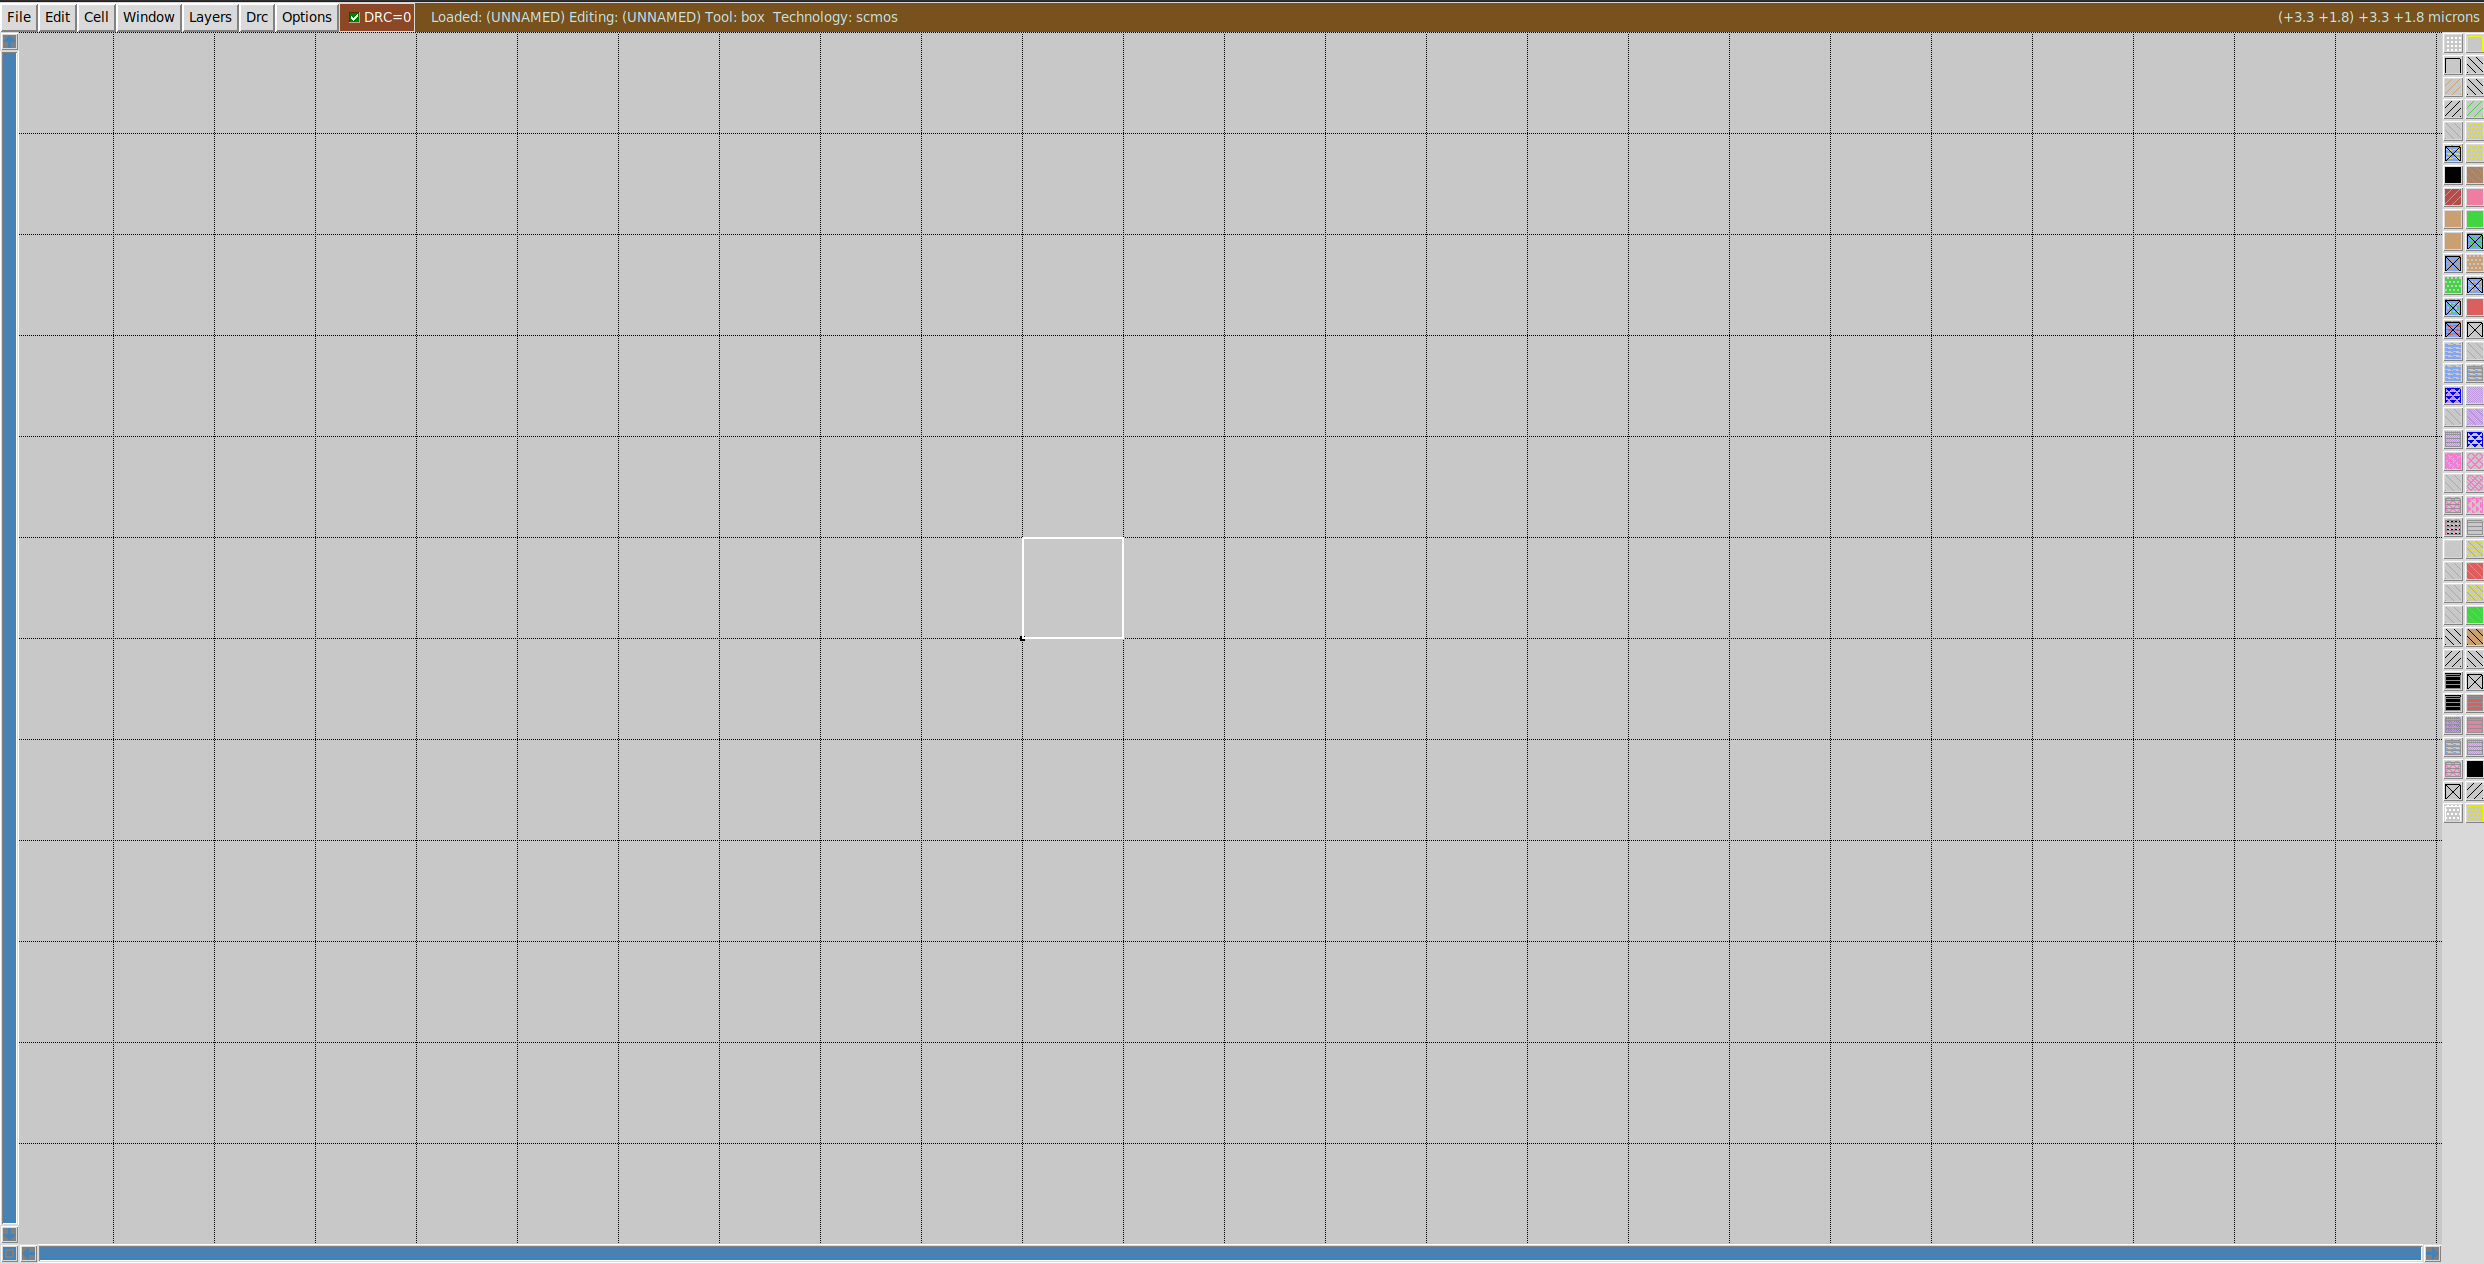
\includegraphics[width=\textwidth]{chapters/chapter2/img/magic_okno}
    \caption{Widok okna programu Magic VLSI.}
    \label{fig:magic_okno}
\end{figure}

\indent Magic VLSI posiada prosty interfejs graficzny,
który składa się z obszaru roboczego, paska narzędzi oraz paska wyboru materiałów.
Dodatkowo wraz z głównym oknem programu otwiera się okno konsoli pozwalające na wprowadzanie dodatkowych komend.
Rysowanie zaczyna się od zaznaczenia obszaru, lewy przycisk myszy służy do wyboru pozycji obszaru,
a prawy do jego rozszerzania.
Aby wypełnić obszar, należy wybrać odpowiedni materiał z paska wyboru
lub z już narysowanych komórek,
poprzez kliknięcie środkowym przyciskiem myszy.
%z tego powodu obecnie można go włączyć jedynie na systemach operacyjnych z rodziny Unix.


\section{Electric}
\section{Microwind}

Microwind to zintegrowane oprogramowanie należące do rodziny EDA (ang. \textit{Electronic Design Automation}),
służące do automatyzacji procesu projektowania układów scalonych lub płytek drukowanych,
umożliwiające projektowanie, symulacje, weryfikacje oraz testowanie układów elektronicznych~\cite{eda}.
Program ten został opracowany przez dra Sicarda do celów edukacyjnych, składa się z kilku modułów,
odpowiadających za różne etapy projektowania układów scalonych~\cite{Microwind}.
Instalacja w przypadku Microwinda jest prosta, wymaga jedynie pobrania pliku instalacyjnego z oficjalnej strony,
a następnie zainstalowania go na komputerze z systemem Windows~\cite{Microwind},
są to natomiast wersje lite (wersja z ograniczoną funkcjonalnością), pełna wersja wymaga licencji.
Dostępna jest także archiwalna pełna wersja programu, która jest dostępna za darmo~\cite{old_microwind}.
Strona zawiera również dokumentację oraz przykłady projektów,
które można wykorzystać w celach edukacyjnych~\cite{Microwind}.\\
\indent Jednym z modułów programu Microwind jest edytor schematów \textbf{Nano Lambda},
pojawiający się domyślnie po uruchomieniu programu.
Posiada dość nieskomplikowany interfejs graficzny z paskiem menu i narzędzi
oraz pływającym oknem palety warstw, przedstawiony na rys.~\ref{fig:microwind_okno}.

\begin{figure}[h]
    \centering
    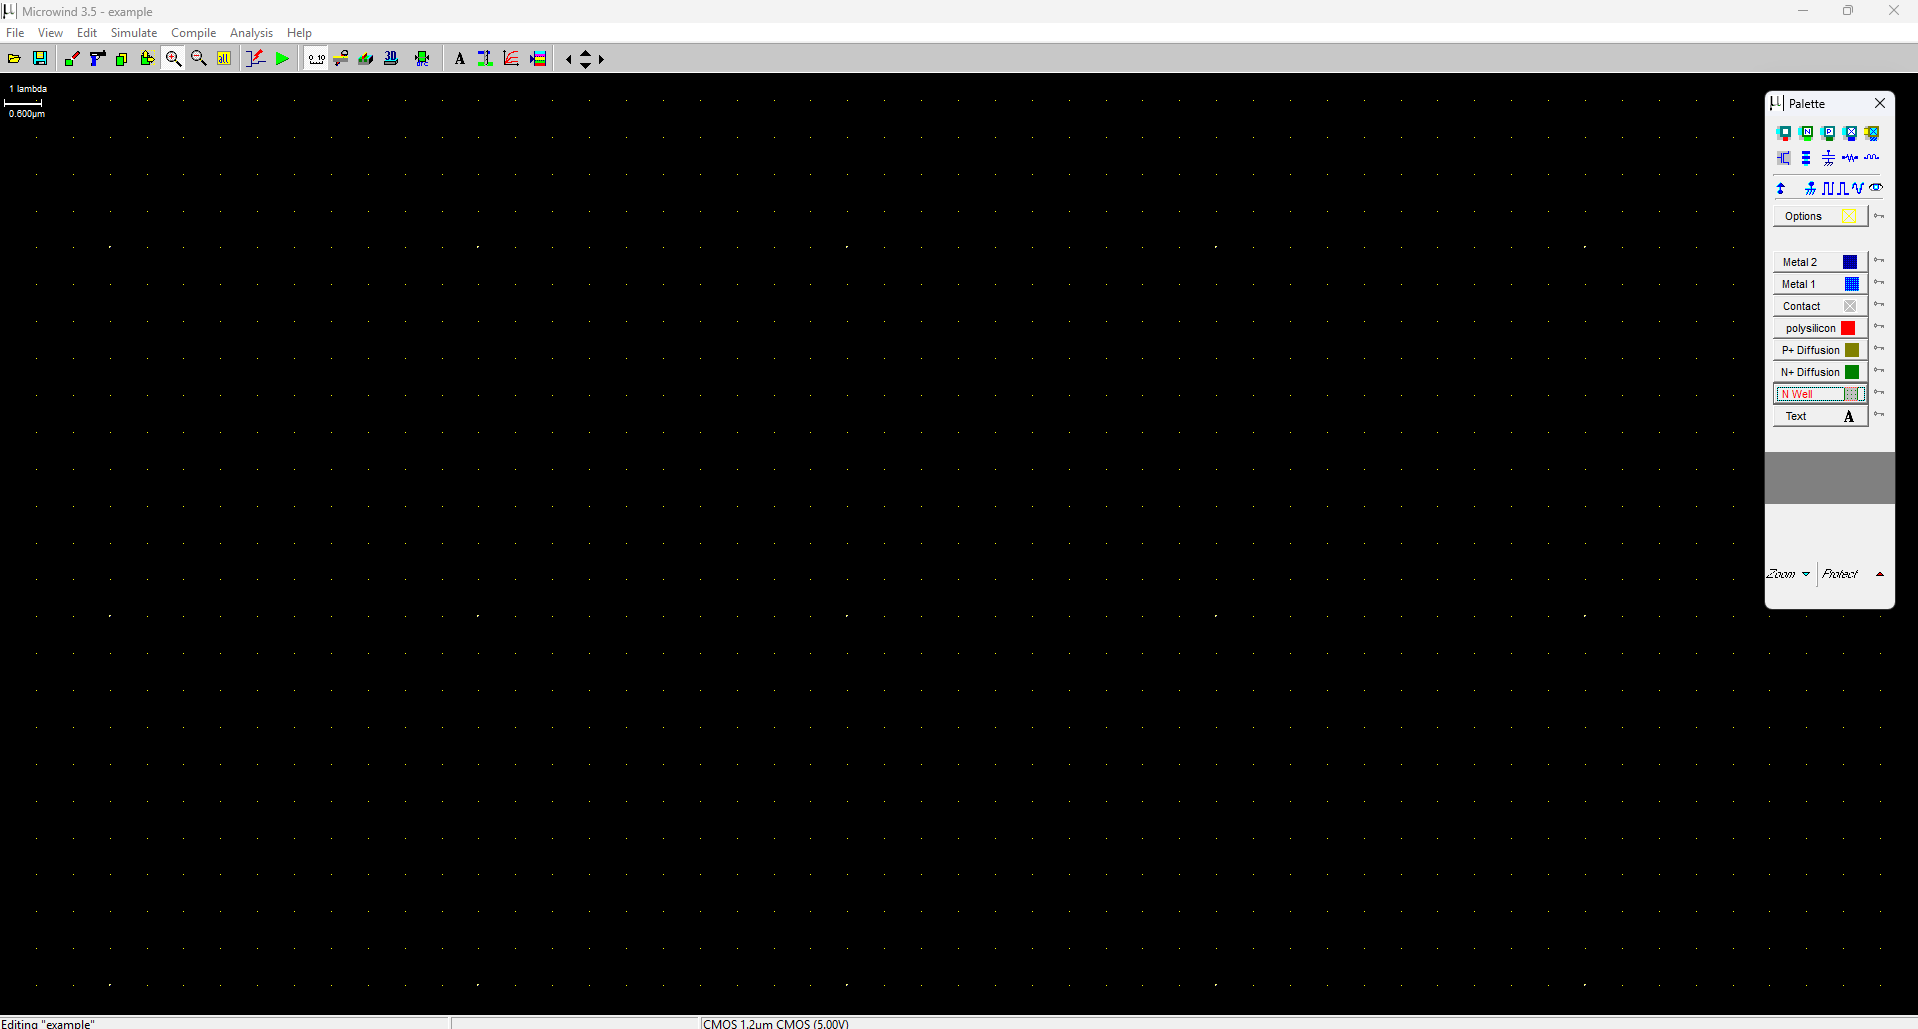
\includegraphics[width=.9\textwidth]{chapters/chapter2/img/microwind_okno}
    \caption[Widok głównego okna programu Microwind.]{Widok głównego okna programu Microwind, źródło:~\cite{Microwind}.}
    \label{fig:microwind_okno}
\end{figure}

\indent Rysowanie odbywa się podobnie jak w przypadku klasycznych edytorów graficznych,
poprzez wybór warstwy z palety,
a następnie przeciągając kursorem po obszarze roboczym przy wciśniętym lewym lub środkowym przycisku myszy,
rysując przy tym prostokątną komórkę.
Nieznaczną wadą rysowania w Microwindzie jest brak przyciągania do siatki,
przez co jest mało precyzyjne.
Przemieszczanie się na obszarze roboczym wymaga używania klawiszy kierunkowych lub przycisków na pasku narzędzi,
co obecnie jest już rozwiązaniem nieergonomicznym.
Program Microwind, poza typowymi narzędziami edycji, charakteryzuje się wieloma zautomatyzowanymi narzędziami,
pozwalającymi generowanie elementów schematów,
na przykład na podstawie funkcji logicznych lub kodu Verilog~\cite{microwind_operation_commands}.\\
\indent Ze względu na brak otwartego kodu źródłowego trudno określić dokładnie zastosowane mechanizmy edytora,
natomiast na podstawie obserwacji można stwierdzić,
że każda edycja schematu wywołuje ponowne rysowanie całego obszaru roboczego,
co jest szczególnie zauważalne podczas usuwania komórek.
Ta sama operacja również wskazuje na strukturę danych, która zakotwiczeniu komórek w kolumnach,
ponieważ po usunięciu obszaru wewnątrz większej komórki, cała kolumna zostaje usunięta.\\
% TODO: poniższe poprawić
\indent Szata graficzna samego edytora charakteryzuje się wysokim kontrastem,
gdzie warstwy są jednolitymi kolorami, częściowo przezroczystymi,
co jest zauważalne, gdy warstwy te się nakładają, przykład przedstawiono na rys.~\ref{fig:microwind_tran}.

\begin{figure}[h]
    \centering
    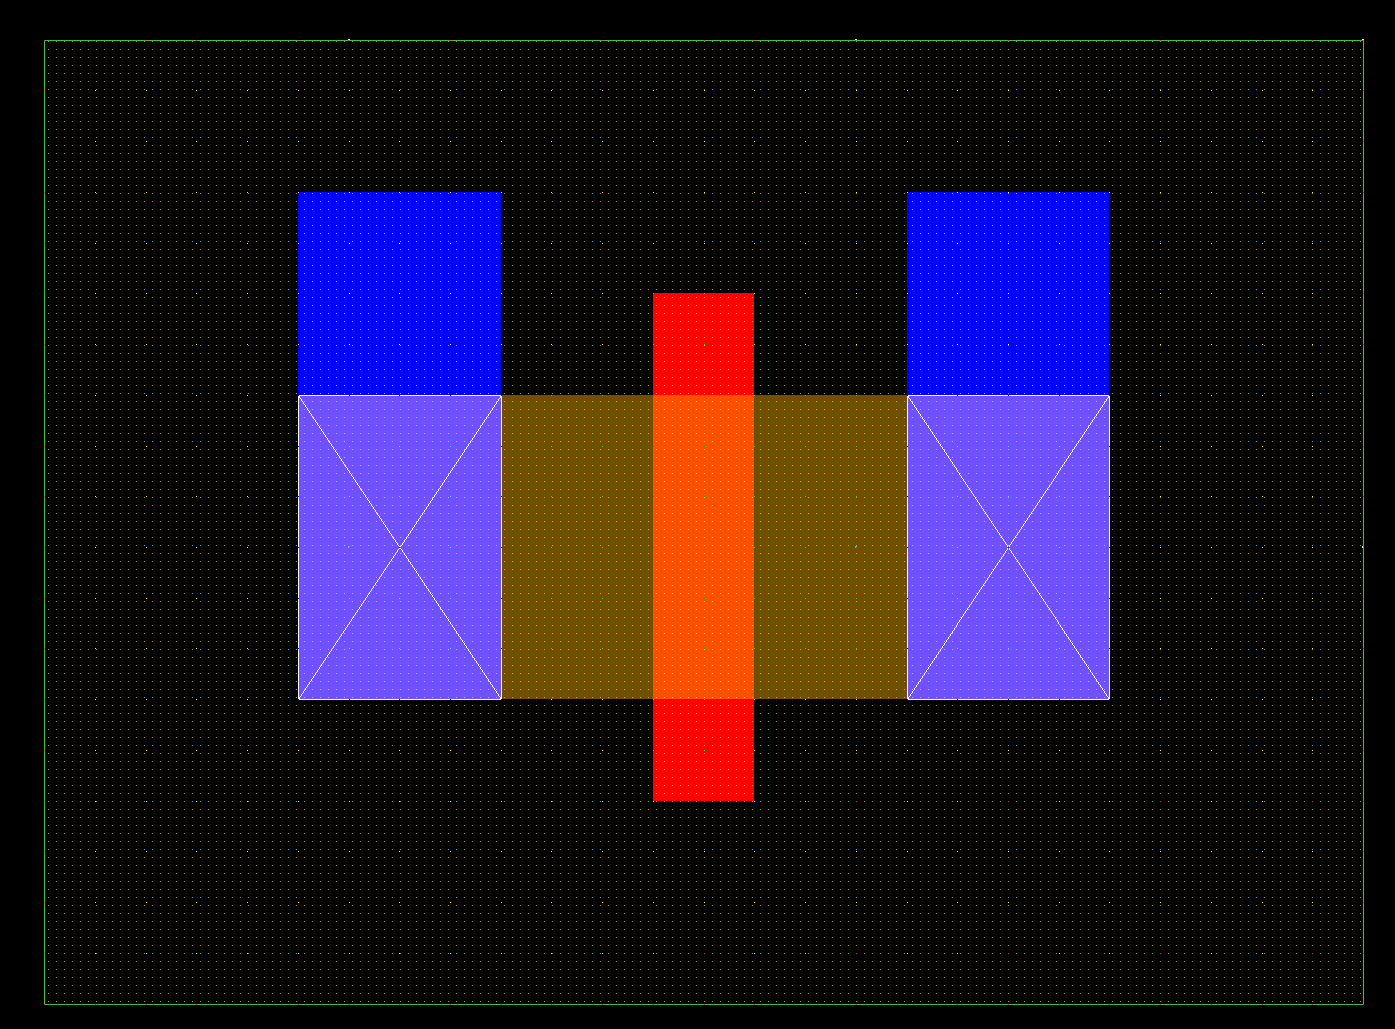
\includegraphics[width=.9\textwidth]{chapters/chapter2/img/microwind_tran}
    \caption[Przykład tranzystora narysowanego w programie Microwind.]
    {
        Przykład tranzystora narysowanego w programie Microwind,
        warstwy \textit{Metal 1}, \textit{P+ Diffusion} oraz \textit{Polysilicon} są jednoilitymi kolorami,
        z wyjątkiem warstwy \textit{N Well} którą reprezentuje kropkowany wzór,
        , źródło: opracowanie własne.
    }
    \label{fig:microwind_tran}
\end{figure}

\chapter{Założenia projektowe}
\label{ch:zalozenia_projektowe}

W przypadku projektowania programu komputerowego, istotne są założenia dla części technicznej oraz funkcjonalnej.
Założenia techniczne określają, jakie technologie i narzędzia zostaną wykorzystane do stworzenia aplikacji,
jak również zastosowane wzorce projektowe oraz architekturę.
Założenia funkcjonalne natomiast mają na celu zdefiniowanie, jakie funkcje i mechanizmy powinny zostać zaimplementowane
oraz przede wszystkim, jak te funkcje pomogą spełnić cel aplikacji.

\section{Założenia funkcjonalne}
\label{sec:zalozenia_funkcjonalne}

Najistotniejsze podczas projektowania programu są założenia funkcjonalne,
które tak naprawdę definiują późniejsze założenia techniczne oraz samo działanie aplikacji.
Założenia te definiują obszary takie jak~interfejs użytkownika, mechanizmy oraz wprowadzanie danych wejściowych.\\
\indent Głównym celem aplikacji jest umożliwienie użytkownikowi projektowanie prostych schematów układów scalonych.
Wymaga to zaimplementowania edytora graficznego będącego w~stanie przedstawić przystępnie topografię układu scalonego.
Najbardziej intuicyjne jest wykorzystanie podejścia opierającego się na rysowaniu komórek,
które składałyby się w~elementy tworzące schemat, podobnie jak~to ma miejsce w~programach Magic VLSI czy Microwind.
Aby wprowadzić podstawowe założenia projektowania układu scalonego, oparto je o technologie Amis C5,
opracowane przez firmę Mosis.
Technologia ta definiuje rzeczywiste wymiary każdej kwadratowej komórki poprzez parametr $\lambda$
zawarty w~regułach projektowania.
Sam wybór jakiejkolwiek technologii projektowania podyktowany
jest próbą nauczenia skalowania wymiarów komórek względem wymiarów rzeczywistych.
Jedne z~takich reguł projektowania to \textit{SCMOS\_SUBM} o $\lambda=0,3~\um$~\cite{amis_c5, amis_params}.
Definiują one również dostępne materiały, z~których może się składać układ, parametry elementów oraz ograniczenia.
Podstawowe materiały przedstawiono w~tab.~\ref{tab:amis_materials}.
Wybór tych materiałów powinien odbywać się poprzez paletę warstw,
dzięki czemu użytkownik może w~sposób prosty wybrać odpowiedni z~nich,
jednocześnie mając przegląd wszystkich dostępnych warstw. 
%Zasady projektowania wskazują także najmniejsze dopuszczalne tranzystory: 3,0\um \times 0,6\um (W/L)~\cite{amis_params}.,
%czyli po podzieleniu przez $\lambda$ otrzymujemy 10 \times 2.

\newpage
\begin{table}[h]
    \centering
    \caption[Dostępne materiały w~technologii Amis C5.]
    {Dostępne podstawowe materiały w~technologii Amis C5, źródło:~\cite{amis_params}.}
    \label{tab:amis_materials}
    \begin{tabular}{|l|l|}
        \hline
        Nazwa materiału & Opis \\
        \hline
        \hline
        \texttt{substrate} & podłoże \\
        \hline
        \texttt{N+active} & inaczej \texttt{ndiffusion}, krzem typu n\\
        \hline
        \texttt{P+active} & inaczej \texttt{pdiffusion}, krzem typu p\\
        \hline
        \texttt{poly} & polikrystaliczny krzem \\
        \hline
        \texttt{poly2} & druga warstwa polikrystalicznego krzemu \\
        \hline
        \texttt{metal1} & pierwsza warstwa metalu \\
        \hline
        \texttt{metal2} & druga warstwa metalu \\
        \hline
    \end{tabular}
\end{table}

Należy zaznaczyć również że~poza samymi warstwami istotne jest także wprowadzenie połączeń między nimi.
Kolejnym istotnym aspektem jest dobór narzędzi edycji schematu.
Powinny one być dostępne w~sposób intuicyjny, być łatwe w~obsłudze oraz umożliwiać większość operacji na schemacie.
Narzędzia te można rozdzielić na dwa rodzaje: narzędzia rysujące oraz narzędzia edytujące. \\
\indent Poza samym edytorem istotne jest także wprowadzenie mechaniki gry.
Ma~ona na celu nauczenie użytkownika podstaw projektowania układów scalonych,
stąd też powinna być maksymalnie prosta tak, aby można było skupić się na nauce i~na~samym,
dość skomplikowanym, procesie projektowania

\subsection{Narzędzia rysujące}
\label{subsec:narzedzia_rysujace}

Rysowanie jest podstawą tworzenia schematu, przez co~powinny one być najprostsze i~najbardziej intuicyjne.
Każde z~narzędzi powinno mieć przypisane skróty klawiszowe,
które przedstawiono wraz z~resztą w~tab.~\ref{tab:key_shortcuts}. % TODO: dodać coś o warstwach i~ich wyborze
Dodanie skrótów klawiszowych pozwoli na zwiększenie efektywności pracy z~edytorem~\cite{shortcuts}
Z~podstawowych narzędzi, jakie mogą być przydatne w~edytorze schematów, można wymienić:

\begin{citemize}
    \item Pędzel -- podstawowe narzędzie rysujące, które pozwala na rysowanie pojedynczych komórek
    i~które ma największą swobodę i~precyzję rysowania,
    \item Prostokąt -- narzędzie rysujące prostokątne obszary, które pozwala na szybkie,
    ale i~precyzyjne rysowanie dzięki dwóm trybom,
    \item Gumka -- działanie podobne do pędzla, ale zamiast rysować, usuwa komórki.
\end{citemize}

\indent Proces rysowania jest podobny do tego w~programach graficznych,
dzięki oparciu o rysowanie komórek, co~pomaga w~łatwym zapoznaniu się z~edytorem.
Przed rysowaniem wybiera się warstwę (podobnie jak~kolor w~programach graficznych) oraz narzędzie rysujące.

\subsection{Narzędzia edytujące}
\label{subsec:narzedzia_edytujace}

Narzędzia edytujące pozwalają na modyfikowanie już narysowanych komórek.
Podstawą jest zaznaczanie komórek do edytowania,
stąd potrzeba narzędzia zaznaczającego.
Opierać się ono powinno na takiej samej zasadzie działania jak~narzędzie rysowania prostokątnego obszaru,
dzięki czemu użytkownik nie musi zapamiętywać kilku różnych mechanizmów.
Dodatkowo powinny istnieć skróty klawiszowe pozwalające na samo modyfikowanie obszaru poprzez dodawanie
oraz odejmowanie zaznaczenia, przedstawiono je w~tab.~\ref{tab:key_shortcuts}.
Zaznaczony obszar można następnie modyfikować, poprzez narzędzie przesuwania.
Operacje te, również będą miały swoje przypisania klawiszy, co~pozwoli na szybsze operowanie na schemacie. \\
\indent Istotnymi funkcjami jest też oznaczanie istotnych miejsc na schemacie, takich jak~kontakty między warstwami,
czy wejście zasilania i~masy.
Mimo tego, że~są one elementami samego schematu i~mogą być narysowane,
to powinny być one wyróżnione poprzez skategoryzowanie jako odrębne narzędzia.
%\indent Istotną funkcją jest także możliwość cofania ostatnich operacji,
%natomiast ze względu na prostotę edytora ilość cofnięć, powinna być ograniczona,
%co~pozwoli także na uproszczenie programu od strony technicznej. % TODO: dodać ilość kroków cofania

\begin{table}[h]
    \centering
    \caption[Skróty klawiszowe używane w~edytorze schematów.]
    {Skróty klawiszowe używane w~edytorze schematów, źródło: opracowanie własne.}
    \label{tab:key_shortcuts}
    \begin{tabular}{|l||l|p{0.66\textwidth}|}
        \hline
        Skrót & \multicolumn{2}{|l|}{Opis} \\
        \hline
        \hline
        \texttt{B} & \multicolumn{2}{|l|}{Pędzel} \\
        \hline
        \texttt{R} & \multicolumn{2}{|l|}{Rysowanie prostokątnego obszaru poprzez przeciąganie} \\
        \cline{2-3}
        & \texttt{Shift} & Przytrzymanie pozwala na rysowanie poprzez wybranie punktu początkowego i~końcowego obszaru \\
        \hline
        \texttt{E} & \multicolumn{2}{|l|}{Gumka} \\
        \hline
        \texttt{W} & \multicolumn{2}{|l|}{Usuwanie prostokątnego obszaru} \\
        \cline{2-3}
        & \texttt{Shift} & Przytrzymanie pozwala na rysowanie poprzez wybranie punktu początkowego i~końcowego obszaru \\
        \hline
        \texttt{S} & \multicolumn{2}{|l|}{Zaznaczanie obszaru poprzez przeciąganie} \\
        \cline{2-3}
        & \texttt{Shift} & Przytrzymanie pozwala na rysowanie poprzez wybranie punktu początkowego i~końcowego obszaru \\
        \cline{2-3}
        & \texttt{Ctrl} & Przytrzymanie pozwala na dodawanie zaznaczenia \\
        \cline{2-3}
        & \texttt{Alt} & Przytrzymanie pozwala na odejmowanie zaznaczenia \\
        \hline
        \texttt{M} & \multicolumn{2}{|l|}{Przesuwanie zaznaczonego obszaru} \\
        \hline
        \texttt{C} & \multicolumn{2}{|l|}{Zaznaczanie kontaktów} \\
        \cline{2-3}
        & \texttt{Shift} & Przytrzymanie pozwala na rysowanie poprzez wybranie punktu początkowego i~końcowego obszaru \\
        \hline
        \texttt{D} & \multicolumn{2}{|l|}{Zaznaczanie zasilania} \\
        \hline
        \texttt{G} & \multicolumn{2}{|l|}{Zaznaczanie masy} \\
        \hline
%        \hline
%        \texttt{Ctrl + Z} & \multicolumn{2}{|l|}{Cofanie ostatniej operacji} \\
%        \hline
%        \texttt{Ctrl + Y} & \multicolumn{2}{|l|}{Ponawianie cofniętej operacji} \\
%        \hline
%        \texttt{Delete} & \multicolumn{2}{|l|}{Usuwanie zaznaczonego elementu} \\
%        \hline
%        \texttt{Ctrl + X} & \multicolumn{2}{|l|}{Wycinanie zaznaczonego elementu} \\
%        \hline
%        \texttt{Ctrl + C} & \multicolumn{2}{|l|}{Kopiowanie zaznaczonego elementu} \\
%        \hline
%        \texttt{Ctrl + V} & \multicolumn{2}{|l|}{Wklejanie skopiowanego/wyciętego elementu} \\
%        \hline
    \end{tabular}
\end{table}\

%\begin{table}[h]
%    \centering
%    \caption[Skróty klawiszowe używane w~edytorze schematów.]
%    {Skróty klawiszowe używane w~edytorze schematów, źródło: opracowanie własne.}
%    \label{tab:key_shortcuts}
%    \begin{tabular}{l l p{0.7\textwidth}}
%        Skrót & \multicolumn{2}{l}{Opis} \\
%        \hline
%        \texttt{B} & \multicolumn{2}{l}{Pędzel} \\
%        \texttt{R} & \multicolumn{2}{l}{Rysowanie prostokątnego obszaru poprzez przeciąganie} \\
%        & \texttt{Shift} & Przytrzymanie pozwala na rysowanie poprzez wybranie punktu początkowego i~końcowego obszaru \\
%        \texttt{S} & \multicolumn{2}{l}{Zaznaczanie obszaru poprzez przeciąganie} \\
%        & \texttt{Shift} & Przytrzymanie pozwala na rysowanie poprzez wybranie punktu początkowego i~końcowego obszaru \\
%        & \texttt{Ctrl} & Dodawanie zaznaczenia \\
%        & \texttt{Alt} & Odejmowanie zaznaczenia \\
%    \end{tabular}
%\end{table}

\subsection{Mechanika gry}
\label{subsec:mechanika_gry}

Mechanika gry ma na celu nauczenie użytkownika podstaw projektowania układów scalonych,
jednocześnie starając się nie skomplikować samego procesu projektowania.
Tak samo, jak~w~grach typu puzzle, gra będzie składać się z~poziomów,
które będą stopniowo wprowadzać użytkownika w~proces projektowania.
Każdy z~poziomów będzie posiadał wymagania w~formie listy komponentów,
gdzie powinny być podłączone oraz jakie mają mieć parametry.
%w~formie schematu elektrycznego oraz opisowej instrukcji.
Gdy użytkownik uzna, że~spełnił wymagania, będzie mógł sprawdzić swoje rozwiązanie,
które zostanie zweryfikowane przez system sprawdzający.
W~przypadku błędów %punktacja za poziom będzie obniżona,
użytkownik będzie mógł poprawić swoje rozwiązanie. %lub rozpocząć poziom od nowa z~pełną pulą punktów.
%Dodatkowo w~trakcie projektowania będzie można sprawdzić, czy dotychczasowy schemat jest poprawny,
%kosztem finalnej punktacji za poziom.
%Aby uniemożliwić nadużywanie tej mechaniki, wprowadzony zostanie limit czasu na jej użycie.
Gdy zatwierdzony schemat spełni wymagania, gracz może przejść do kolejnego poziomu.
Przepływ rozgrywki dokładniej przedstawiono w~tab.~\ref{tab:game_flow}.

\begin{table}[h]
    \centering
    \caption[Przepływ rozgrywki.]
    {Przepływ rozgrywki, źródło: opracowanie własne.}
    \label{tab:game_flow}
    \begin{tabular}{|l p{0.22\textwidth}|p{0.6\textwidth}|}
        \hline
        \multicolumn{2}{|l|}{Krok} & Opis \\
        \hline
        \hline
        1 & Rozpoczęcie poziomu &
        Użytkownik rozpoczyna poziom, przedstawia się mu wymagania w~formie listy wymaganych komponentów. \\
        \hline
        2 & Projektowanie schematu &
        Użytkownik projektuje schemat\\ %, w~ograniczonym czasie może sprawdzać jego poprawność kosztem punktów. \\
        \hline
        3 & Weryfikacja schematu &
        Użytkownik zatwierdza schemat, który następnie zostaje sprawdzony przez system. \\
        \hline
        4 & Wynik &
        Gracz dostaje informacje czy wymagania zostały spełnione, czy nie. \\
        \hline
        5a & Wynik pozytywny &
        Wymagania zostały spełnione, gracz może przejść do kolejnego poziomu. \\
        \hline
        5b & Wynik negatywny &
        Wymagania nie zostały spełnione, gracz może poprawić schemat. \\
        \hline
    \end{tabular}
\end{table}

%\begin{table}[h]
%    \centering
%    \caption[Przepływ rozgrywki.]
%    {Przepływ rozgrywki, źródło: opracowanie własne.}
%    \label{tab:game_flow}
%    \begin{tabular}{l p{0.22\textwidth} p{0.6\textwidth}}
%        \multicolumn{2}{l}{Krok} & Opis \\
%        \hline
%        1 & Rozpoczęcie poziomu &
%        Użytkownik rozpoczyna poziom, przedstawia się mu wymagania w~formie schematu elektrycznego oraz opisu. \\
%        2 & Projektowanie schematu & 
%        Użytkownik projektuje schemat, w~ograniczonym czasie może sprawdzać jego poprawność kosztem punktów. \\
%        3 & Weryfikacja schematu &
%        Użytkownik zatwierdza schemat, który następnie zostaje sprawdzony przez system. \\
%        4 & Wynik &
%        Gracz dostaje informacje czy wymagania zostały spełnione, czy nie. \\
%        5a & Wynik pozytywny &
%        Wymagania zostały spełnione, gracz może przejść do kolejnego poziomu. \\
%        5b & Wynik negatywny &
%        Wymagania nie zostały spełnione, gracz może poprawić schemat lub rozpocząć poziom od nowa. \\
%    \end{tabular}
%\end{table}

%\subsection{Podsumowanie założeń funkcjonalnych}
%\label{subsec:podsumowanie_zalozen_funkcjonalnych}
%
%Założenia funkcjonalne są kluczowe dla projektu, gdyż definiują one obszary, na które należy zwrócić szczególną uwagę.


\section{Założenia techniczne}
\label{sec:zalozenia_techniczne}

Ze względu na charakter aplikacji, jakim jest edukacyjna gra komputerowa,
opierająca się w dużym stopniu na renderowaniu grafiki,
do wykonania projektu wybrano silnik Unity w wersji 6000.0.25f1~\cite{unity_site}.
Z wielu zalet silnika Unity, kluczowe dla niniejszego projektu są:

\begin{citemize}
    \item Wsparcie dla wielu platform --
    Unity pozwala na tworzenie aplikacji na wiele platform jednocześnie, w tym przede wszystkim na systemy Windows, Linux oraz macOS.
    \item Prostota tworzenia aplikacji graficznych --
    Unity oferuje wiele narzędzi, które ułatwiają tworzenie interaktywnych aplikacji graficznych,
    dzięki czemu można skupić się na tworzeniu mechanik gry.
    \item Szerokie wsparcie --
    Unity posiada rozbudowaną dokumentację~\cite{unity_docs},
    aktywne forum~\cite{unity_forum} oraz wiele darmowych zasobów.
\end{citemize}


Unity korzysta z języka C\#,
który bazuje na paradygmacie programowania obiektowego (ang. OOP — Object-Oriented Programming).
OOP opiera się na definiowaniu klas jako abstrakcji oraz tworzeniu ich instancji,
a także na współpracy między nimi~\cite{nygaard1986basic}.
Dzięki temu można tworzyć obiekty o wspólnych cechach,
co znacząco upraszcza pisanie kodu i jego późniejszą konserwację.\\
%Unity korzysta z języka C\#, opartego o paradygmat programowania obiektowego (ang. OOP -- Object-Oriented Programming),
%polegający na tworzeniu obiektów na podstawie abstrakcji klas, a także innych obiektów~\cite{nygaard1986basic}.
%Pozwala to na tworzenie wielu obiektów o podobnych cechach, co ułatwia pisanie kodu oraz jego późniejsze utrzymanie.\\
\indent Programowanie w silniku Unity opiera się na tzw. \textit{MonoBehaviour},
który jest klasą bazową dla większości skryptów w Unity.
Klasa ta pozwala na dostęp do informacji, jakie zawiera \textit{GameObject} oraz jego komponentów.
\textit{GameObject} jest natomiast Unitowym odpowiednikiem obiektu w edytorze,
składają się na niego komponenty, które odpowiadają za różne funkcje, jakie on pełni,
w tym przede wszystkim \textit{Transform}, który wskazuje pozycję, rotację oraz skalę obiektu.\\
\indent Kolejnym istotnym elementem w Unity są sceny,
które pozwalają na posiadanie wielu kilku różnych środowisk w jednym projekcie.
Sceny te mogą być wykorzystane do okna startowego oraz okna edytora schematu.
Resztę elementów można wykonać jako odrębne okienka w interfejsie użytkownika w danej scenie.
Wygląd edytora Unity przedstawiono na rys.~\ref{fig:unity_editor}.

\begin{figure}[h]
    \centering
    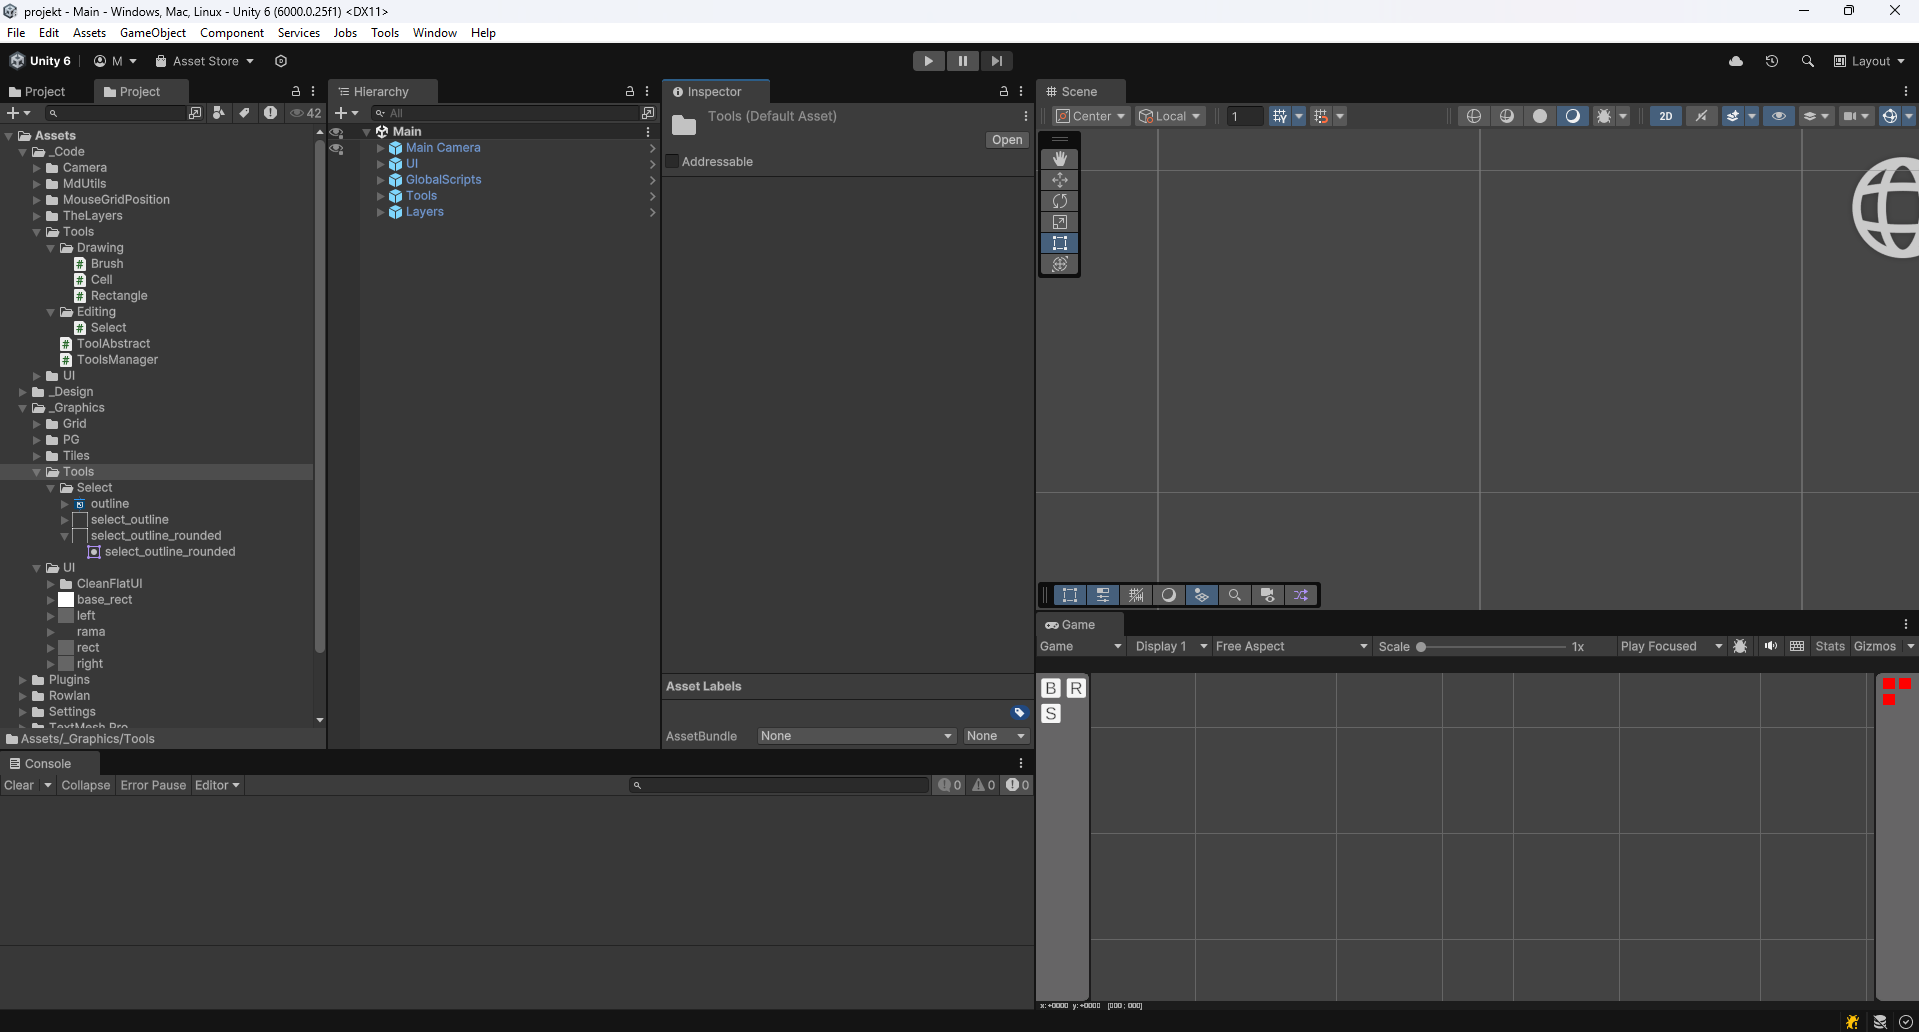
\includegraphics[width=0.9\textwidth]{chapters/chapter3/rys/unity_editor}
    \caption[Widok okna edytora Unity]{Wygląd edytora Unity, źródło: \cite{unity_site}}
    \label{fig:unity_editor}
\end{figure}

\subsection{Architektura programu}
\label{subsec:architektura_programu}

Aby zapewnić modularność oraz separację elementów aplikacji,
wykorzystano odpowiednio zaadaptowana architekturę MVVM (ang. Model-View-ViewModel).
Polega ona na podziale na trzy główne części: model, widok oraz widok-model.
Funkcje każdego z nich opisano w tab.~\ref{tab:mvvm}.

\begin{table}[h]
    \centering
    \caption[Opis funkcji poszczególnych elementów architektury MVVM.]
    {Opis funkcji poszczególnych elementów architektury MVVM, źródło:~\cite{mvvm}.}
    \label{tab:mvvm}
    \begin{tabular}{|c|p{0.6\textwidth}|}
        \hline
        Element & Opis \\
        \hline
        \hline
        Widok & Odpowiada za prezentację danych oraz interakcję z użytkownikiem. \\
        \hline
        Widok-model & Odpowiada za przekazywanie danych pomiędzy modelem a widokiem. \\
        \hline
        Model & Odpowiada za przechowywanie danych oraz logikę danego komponentu programu. \\
        \hline
    \end{tabular}
\end{table}

%Tak jak pierwotnie w architekturze MVVM,
%widok odpowiada za prezentację danych oraz interakcję z użytkownikiem.
%Przy czym po adaptacji widok-model odpowiada za nie tylko przekazywanie danych nie tylko między modelem a widokiem,
%ale również pomiędzy innymi częściami aplikacji jako menedżer danego systemu aplikacji.
%Sam model natomiast składa się z wielu komponentów, które przechowują dane oraz logikę danego komponentu aplikacji.
Przy większych projektach model ten jest stosowany do większości komponentów składających się na aplikację.
Widok-model w tej sytuacji odpowiada za przekazywanie danych nie tylko między modelem a widokiem,
ale również pomiędzy innymi częściami wewnątrz aplikacji jako menedżer danego systemu.
W przypadku opracowywanego programu można wyróżnić cztery główne systemy dotyczące różnych aspektów aplikacji:

\begin{citemize}
    \item System zarządzania progresem gry, odpowiadający za kontrolę przebiegu gry,
    a także punktację oraz weryfikację poziomów,
    \item Narzędzia do rysowania i edycji, wybieranie ich oraz kontrola ich działania,
    \item System zarządzania rysowanym schematem,
    odpowiadający za renderowanie warstw i przechowywanie informacji o nich
    oraz kontrolujący ich widok czy połączenia, na jakie się składają,
    \item System zapisu, odpowiadający za zapis i odczyt stanu gry.
\end{citemize}

%zarządzanie progresem gry, narzędzia do rysowania i edycji, system zarządzania rysowanym schematem, oraz system zapisu.
Odstępstwem od architektury MVVM jest natomiast potrzeba bezpośredniej interakcji pomiędzy użytkownikiem
a narzędziami ze względu na ich różnorodność, co przekłada się także na mniej skomplikowany kod.\\
Zarys architektury programu przedstawiono na rys.~\ref{fig:architektura}.

\begin{figure}[h!]
    \centering
    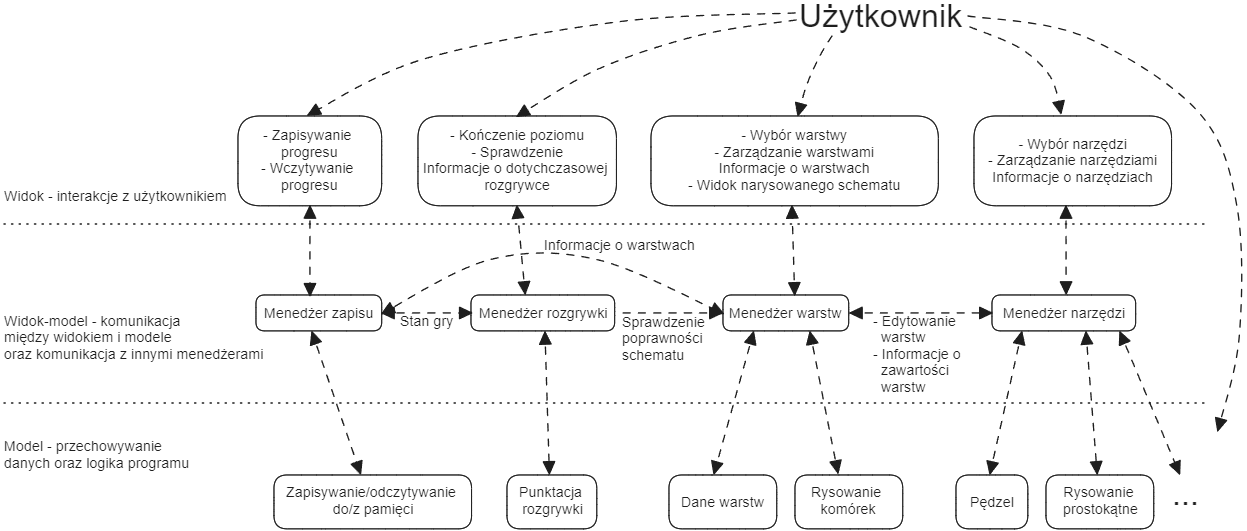
\includegraphics[width=\textwidth]{chapters/chapter3/rys/arch}
    \caption[Architektura programu.]{Architektura programu, źródło: opracowanie własne.}
    \label{fig:architektura}
\end{figure}

%\newpage % TODO: check this if something changes
\subsection{Wykorzystanie funkcji Unity oraz paczek zasobów}
\label{subsec:zasoby}

Do rysowania komórek schematów wykorzystano komponent \textit{SpriteRenderer},
pozwalający na renderowanie dwu-wymiarowych obrazów nazywanych \textit{sprite'ami}.
Dużą zaletą tego komponentu jest wbudowana optymalizacja ze strony Unity.
Obiektów tego typu może być wiele na scenie oraz są one renderowane tylko,
gdy są widoczne na ekranie~\cite{unity_csharp, unity_docs}. \\
\indent Prócz podstawowego skryptu, na jakim bazuje Unity, czyli \textit{MonoBehaviour},
wykorzystano także \textit{ScriptableObject}.
Jest to klasa, która pozwala na tworzenie obiektów, które mogą przechowywać dane zdefiniowane poza pracą programu,
a nawet wykonywać prostą logikę~\cite{unity_csharp, unity_docs}.
%Pozwala to na szczególną modularność dzięki możliwości wcześniejszego zdefiniowania danych zawartych w obiekcie
%i co mają one robić, a następnie tworzenie obiektów na ich podstawie.
Działanie SO jest zbliżone do klas i obiektów w OOP,
przy czym SO jest wykorzystywany przede wszystkim w edytorze Unity.
Dzięki temu można wcześniej zdefiniować jaki rodzaj danych powinien przechowywać dany typ obiektu,
a następnie tworzyć na ich podstawie konkretne instancje, których dane można zmieniać w edytorze.
Zostało to w szczególności wykorzystane w systemach zarządzania, rysowanym schematem
i narzędziami do rysowania i edycji.\\
%W przypadku schematu SO przechowuje informacje o tym jak powinny wyglądać i zachowywać się warstwy,
%natomiast do narzędzi SO zostały wykorzystane jako konfiguracje 
\indent W celu optymalizacji wskazane jest korzystanie z asynchroniczności w programie.
W szczególności jest to istotne podczas rysowania lub modyfikowania większych obszarów,
ponieważ wymaga to działania na wielu komórkach.
Skorzystano tutaj z paczki zasobów \textit{UniTask} do obsługi asynchroniczności,
dostępnej na platformie GitHub~\cite{unitask}.
Paczka ta adaptuje wbudowany w C\# system asynchroniczności,
dzięki czemu jest on znacznie optymalniejszy pod kątem wykorzystania w silniku Unity.


\subsection{Interfejs użytkownika}
\label{subsec:interfejs_uzytkownika}

Interfejs użytkownika (ang. \textit{User Interface}) jest jednym z kluczowych elementów każdej aplikacji,
kluczowe jest, aby był on intuicyjny oraz przejrzysty tak,
aby użytkownik mógł skupić się na korzystaniu z programu.
W przypadku opracowywanej aplikacji należy rozdzielić ją na dwie warstwy,
edytor schematów oraz część dotyczącą gry.
Jako że przez większość pracy w programie użytkownik ma do czynienia z edytorem schematów,
jest on podstawowym widokiem.
Z kolei elementy interfejsu dotyczące gry powinny być w formie nakładki na edytor schematów,
z wyjątkiem okna startowego, który będzie odrębną sceną, przez co nie ma potrzeby tworzenia nakładki.
Zarys widoku okna edytora schematów przedstawiono na rys.~\ref{fig:editor}.

\begin{figure}[h]
    \centering
    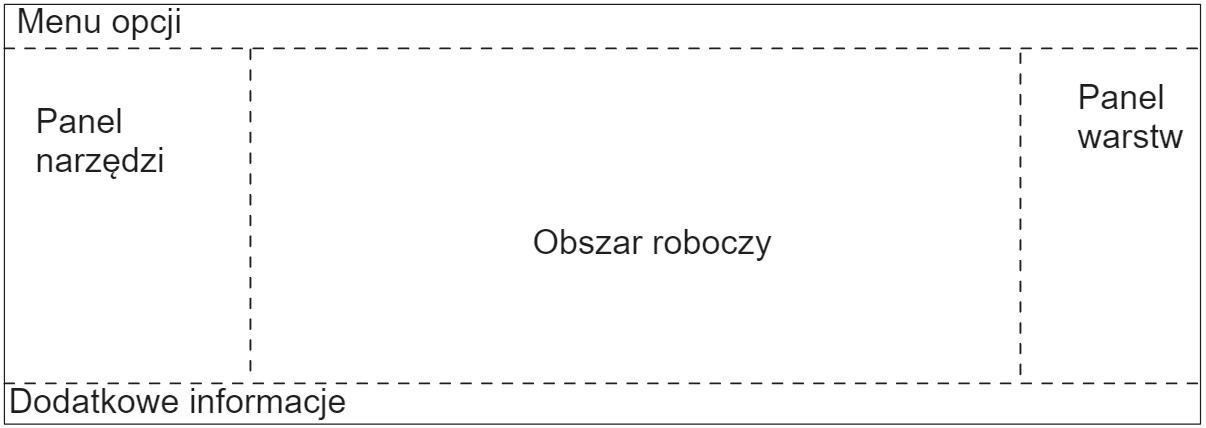
\includegraphics[width=0.89\textwidth]{chapters/chapter3/rys/ui_projekt}
    \caption[Szkic okna edytora schematów]{Szkic okna edytora schematów, źródło: opracowanie własne.}
    \label{fig:editor}
\end{figure}

\indent Okno dla edytora adaptuje elementy
z programów wspomnianych w rozdziale~\ref{ch:przeglad_istniejacych_rozwiazan}.
Tak jak w przypadku większości rozwiązań u góry okna znajduje się pasek opcji programu,
implementujący również opcje związane z grą.
Poniżej znajduje się obszar roboczy, gdzie użytkownik może rysować schematy.
Na dole okna znajduje się pasek informacyjny, który zawiera dane o aktualnie wybranym narzędziu,
a także o możliwych dodatkowych akcjach do wykonania.
Z prawej strony okna znajduje się panel warstw, zawierający dostępne warstwy schematu,
a także dodatkowe informacje o nich wraz z możliwością wyłączenia ich widoczności.
Po lewej usytuowany jest panel narzędzi, zawierający dostępne funkcje rysowania i edycji schematów
i dostępne dla nich opcje.

\chapter{Realizacja projektu}
\label{ch:realizacja_projektu}

Opracowywanie programu w przypadku korzystania z Unity jest częściowo podzielone między warstwę kodu a warstwę projektową,
która obejmuje zarządzanie zasobami, scenami, prefabami oraz innymi elementami, które nie są bezpośrednio związane z kodem.
Natomiast obie są ze sobą ściśle powiązane, kod definiuje komponenty i ich zachowanie,
podczas gdy w edytorze należy odpowiednio skonfigurować te komponenty, aby działały zgodnie z założeniami.
W związku z tym przy opisie każdej części aplikacji należy uwzględnić zarówno aspekty kodowe, jak i projektowe.\\
\indent Zwracając uwagę na architekturę programu, z najistotniejszych elementów do zaprojektowania można wyróżnić:

\begin{citemize}
    \item System zarządzania warstwami, ryoswaniem ich oraz przechowywaniem informacji o nich,
    \item Narzędzia do rysowania i edycji, oraz zarządzanie nimi
    \item System zarządzania progresem gry, a przede wszystkim algorytm weryfikujący poprawność schematów,
    \item Interfejs graficzny pozwalający na interakcję użytkownika z programem, wybór warstw oraz narzędzi.
\end{citemize}

\section{Warstwy oraz ich rysowanie}
\label{sec:warstwy_oraz_ich_rysowanie}

Ponieważ warstwy, oraz ich rysowanie są kluczowymi elementami, definiującymi działanie reszty programu,
a zarazem stanowią najbardziej obciążającą komputer część projektu,
należało rozpatrzyć najoptymalniejsze rozwiązania do zaimplementowania.
Podstawowym założeniem jest przedstawienie komórki na schemacie jako \textit{GameObject} zawierający dwuwymiarowe,
kwadratowe sprite'y,
stąd cały obszar roboczy jest przedstawiony jako siatka.
W związku z tym najprostszy sposób do zapisania danych warstwy to tablica dwuwymiarowa,
gdzie każdy element tablicy odpowiada jednemu kwadratowi na siatce.
%Jeszcze lepiej podzielić taką tablicę na kilka mniejszych oraz przenieść ją do jednego wymiaru.
Dodatkowo w celu optymalizacji taką tablicę można podzielić na kilka mniejszych,
odpowiedzialnych za różne obszary, a także zamienić je na tablice jednowymiarowe.
Rozwiązanie takie pozwala na optymalniejsze zarządzanie pamięcią,
ponieważ całą warstwę można zapisać jako tablice bitów,
gdzie każdy bit odpowiada jednej komórce i \texttt{1} oznacza,
że jest zajęta a~\textt{0} -- wolna.
W połączeniu z tym rozwiązaniem można wykorzystać dwie metody rysowania warstw:

\begin{citemize}
    \item Rysowanie co modyfikację całej warstwy od nowa -- w tej metodzie cała warstwa jest rysowana od nowa po każdej modyfikacji,
    nie ma potrzeby sprawdzania każdego kwadratu czy jest zajęty, oraz pozwala na pośrednie modyfikowanie narysowanej warstwy,
    bez potrzeby posiadania referencji do obiektów na scenie.
    Wadą jest jednak rysowanie całej warstwy po każdej modyfikacji,
    co przy dużym obszarze roboczym i dużej ilości już narysowanych elementów wpłynie negatywnie na optymalizację.
    \item Rysowanie tylko zmienionych kwadratów -- w tej metodzie komórki są rysowane tylko wtedy, gdy są puste,
    co w ogólnym rozrachunku jest szybsze, jednak wymaga sprawdzania każdej komórki czy nie jest zajęta,
    oraz w celu modyfikacji już istniejących elementów, potrzebne jest posiadanie referencji do GO na scenie.
\end{citemize}

%rysowanie co zmianę całości od nowa, dzięki czemu nie trzeba sprawdzać każdego kwadratu czy już jest zajęty,
%oraz rysowanie tylko zmienionych kwadratów, co w ogólnym rozrachunku jest szybsze,
%natomiast wymaga sprawdzanie każdej komórki czy nie jest zajęta,
%aby nie doszło do sytuacji, gdzie sprite'y się nakładają.
Niestety powyższe rozwiązania wymagają ciągłego iterowania po całej tablicy nawet przy modyfikacji jednego elementu
i albo dodatkowego przetrzymywania referencji, albo ciężkiego obliczeniowo rysowania całej warstwy od nowa.
W związku z tym wybrano inne rozwiązanie, polegające na wykorzystaniu systemu fizyki w silniku Unity,
który pozwala na wykrywanie kolizji pomiędzy obiektami.
Pozwala to na niezależne wykrywanie komórek bez potrzeby referencji do nich,
znacząco upraszczając zarządzanie nimi oraz proces rysowania.
W tym celu do obiektu komórki prócz komponentu \texttt{SpriteRenderer} dodano komponent \texttt{BoxCollider},
dzięki czemu obiekt ten może być wykrywany przez system fizyki.\\
\indent Kolejny sposobem na optymalizację jest wykorzystanie puli obiektów.
Ponieważ w wielu przypadkach potrzebne będzie stworzenie wielu obiektów naraz, co jest kosztowne obliczeniowo,
w trakcie działania programu co klatkę tworzy się ich tylko kilka nieaktywnych, które są następnie przechowywane w puli.
Gdy potrzebny jest nowy obiekt, pobiera się go z puli i aktywuje, a gdy nie jest już potrzebny,
zamiast go usuwać, jest on dezaktywowany i przenoszony z powrotem do puli.
Do implementacji tego mechanizmu dla komórek stworzono komponent \texttt{CellsPool},
posiadający listę struktur \texttt{PoolData} dla każdej z warstw.
Struktura ta przechowuje informację o tym, dla jakiej warstwy jest pula oraz samą pulę obiektów.
Do przetrzymywania tworzonych GO wykorzystano klasę \texttt{Queue},
jest to struktura danych FIFO (ang. \textit{First In, First Out}),
która pozwala na dodawanie elementów na koniec kolejki oraz usuwanie z jej początku.
Aby uporządkować w hierarchii w edytorze wszystkie tworzone w puli obiekty,
jako swojego rodzica mają ustawiony obiekt \texttt{CellsPool}\\
\indent Do definiowania warstw stworzono \texttt{ScriptableObject} \texttt{LayerConfig}.
Zawiera on informacje o nazwie warstwy, jej kolejności na schemacie, jaki sprite ma być rysowany, kolor,
zasady projektowania (minimalna odległość między niesąsiadującymi komórkami, minimalna szerokość)
oraz maksymalną wielkość puli komórek.
Dzięki temu można w łatwy sposób tworzyć nowe warstwy, a także modyfikować definicje już istniejących.
Dodatkowo \texttt{LayerConfig} jest używany jako klucz do identyfikacji warstwy w innych komponentach.
Przykład takiej konfiguracji przedstawiono na rys.~\ref{fig:layer_config}.

\begin{figure}[h]
    \centering
    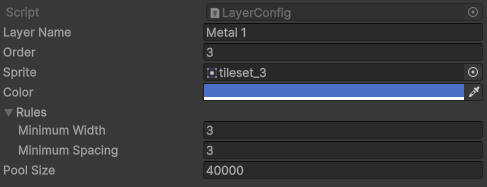
\includegraphics[width=.9\textwidth]{chapters/chapter4/rys/layer_config}
    \caption[Przykładowe okno konfiguracji warstwy \textit{Metal 1}.]
    {Przykładowe okno konfiguracji warstwy \textit{Metal 1}, źródło: opracowanie własne.}
    \label{fig:layer_config}
\end{figure}

%\newpage % TODO: check this if something changes

\indent W trakcie działania programu wszystkie narysowane komórki danej warstwy
są przechowywane w komponencie \texttt{LayerHolder} jako lista obiektów \texttt{GameObject}.
Komponent ten jest także w głównej mierze odpowiedzialny za rysowanie
i usuwanie pojedynczych komórek poprzez metody \texttt{NewCell} oraz \texttt{ReturnCell}.
a także umożliwia dostęp do wszystkich komórek danej warstwy.
Inicjalizacją \texttt{LayerHolder} zajmuje się \texttt{LayersManager}, podczas startu programu.
Z jego głównych funkji można wymienić:

\begin{citemize}
    \item Tworzenie warstw na podstawie konfiguracji z \texttt{LayerConfig},
    \item Przechowywanie referencji do wszystkich warstw,
    \item Wybór oraz zwracanie obecnie rysowanej warstwy,
    \item Włączanie i wyłączanie warstw,
    \item Pośredniczenie przy zwracaniu komórek do puli.
\end{citemize}

Ze względu na istotność tego komponentu, zdecydowano się na zastosowanie wzorca projektowego \textit{Singleton},
dzięki czemu jest on dostępny z każdego miejsca w programie
oraz implikuje posiadanie tylko jednej instancji tego obiektu w trakcie działania programu.
W przypadku Unity, ze względu na to, że klasą bazową komponentów jest \texttt{MonoBehaviour},
należało zaimplementować wzorzec poprzez opracowanie klasy \texttt{MonoSingleton},
której kod przedstawiono na listingu~\ref{lst:monosingleton}.

\begin{lstlisting}[language={C},label=lst:monosingleton,caption={Klasa \texttt{MonoSingleton}}]
public class MonoSingleton<T> : MonoBehaviour where T : Component {
    public static T Instance => _instance;
    private static T _instance;
    protected void Awake() {
        if (_instance != null && _instance != this as T)
            throw new Exception($"Singleton already exists! : {_instance.name}");
        _instance = this as T;
    }
}
\end{lstlisting}

\input{chapters/chapter4/}

% Bibliography
\bibliography{main}
\bibliographystyle{unsrt}
\addcontentsline{toc}{chapter}{Bibliografia}
    
% List of figures
\thispagestyle{empty}
\listoffigures
\addcontentsline{toc}{chapter}{Spis rysunków}
    
% List of tables
\thispagestyle{empty}
\listoftables
\addcontentsline{toc}{chapter}{Spis tabel}

\end{document}
